\subsection{Efficiency}\label{sec:WBoson_Analysis_Efficiency}

This section describes the procedure used to derive and correct the muon efficiency of \WToMuNu signal events.

\subsubsection{MC Truth Efficiency}\label{sec:WBoson_Analysis_MCTruthEfficiency}

In order to estimate the signal efficiency, the \WToMuNu MC samples listed in \tab{tab:MCSamples} are used since they contain the full history of the events, including the generation and reconstruction of the particles. The energy deposited in the HF calorimeters of the simulated events is reweighted to match the distribution observed in data as explained in \sect{sec:WBoson_Analysis_EventActivityReweighting}.

A reconstructed muon is considered an offline muon if it passes all the \W analysis cuts. Among the selection criteria, an offline muon is required to pass the isolation and tight identification cuts defined in \sect{sec:WBoson_Analysis_ObjectReconstruction}, be trigger matched as explained in \sect{sec:WBoson_Analysis_MuonTrigger}, and have a $\pt~>~25$~\GeVc and $|\eta|~<~2.4$.

The muon truth efficiency is defined as the fraction of generated muons matched to an offline muon according to \sect{sec:WBoson_Analysis_GenRecoMatching}.  All the generated muons are required to be inside the analysis kinematic region ($\pt~>~25$~\GeVc and $|\eta|~<~2.4$) and come from a \W boson decay. The muon efficiency is described in \eq{eq:MCTruthEfficiency}.

\begin{equation}
\epsilon^{\mu^{\pm}}_{offline}(p_{T}^{gen} , \eta^{gen}) = \frac{N_{gen,\pt>25}^{\mu^{\pm}}(p_{T}^{gen} , \eta^{gen})[\textnormal{Matched to }\mu_{offline}^{\pm}]}{N_{gen,\pt>25}^{\mu^{\pm}}(p_{T}^{gen} , \eta^{gen})}
\label{eq:MCTruthEfficiency}
\end{equation}

The muon efficiencies of the \pPb and \Pbp MC samples are calculated individually and later combined following the strategy described in \sect{sec:WBoson_Analysis_CombiningBeamDirection}. After flipping the sign of the muon $\eta_{LAB}$ in the \Pbp sample, the combined efficiency is determined as presented in \eq{eq:MCEfficiencyPA} by taking into account the corresponding recorded integrated luminosities of each run (see \sect{sec:WBoson_Analysis_DataSamples}). The combined efficiency is labelled as pA muon efficiency.

\begin{equation}
\epsilon^{\mu^{\pm}}_{PA}(p_{T}^{gen} , \eta^{gen}) = \frac{\sigma^{MC}_{\pPb}\times\Lumi_{\pPb}\times\epsilon^{\mu^{\pm}}_{\pPb}(p_{T}^{gen} , \eta^{gen}) + \sigma^{MC}_{\Pbp}\times\Lumi_{\Pbp}\times\epsilon^{\mu^{\pm}}_{\Pbp}(p_{T}^{gen} , -\eta^{gen})}{\sigma^{MC}_{\pPb}\times\Lumi_{\pPb} + \sigma^{MC}_{\Pbp}\times\Lumi_{\Pbp}}
\label{eq:MCEfficiencyPA}
\end{equation}

The statistical uncertainty of the computation of the muon efficiencies is determined using the ROOT class TEfficiency \cite{ROOT}. The uncertainty is estimated by applying Bayesian statistics using a Jeffrey's prior and considering a 68$\%$ credible interval. The results of the \WToMuNu truth efficiency extracted from the combined pA MC samples are shown in \fig{fig:MCTruthEfficiency} and in \tab{tab:mcEfficiency_WToMu_PA}, as function of $\eta_{CM}$.

\begin{figure}[htb!]
 \begin{center}
   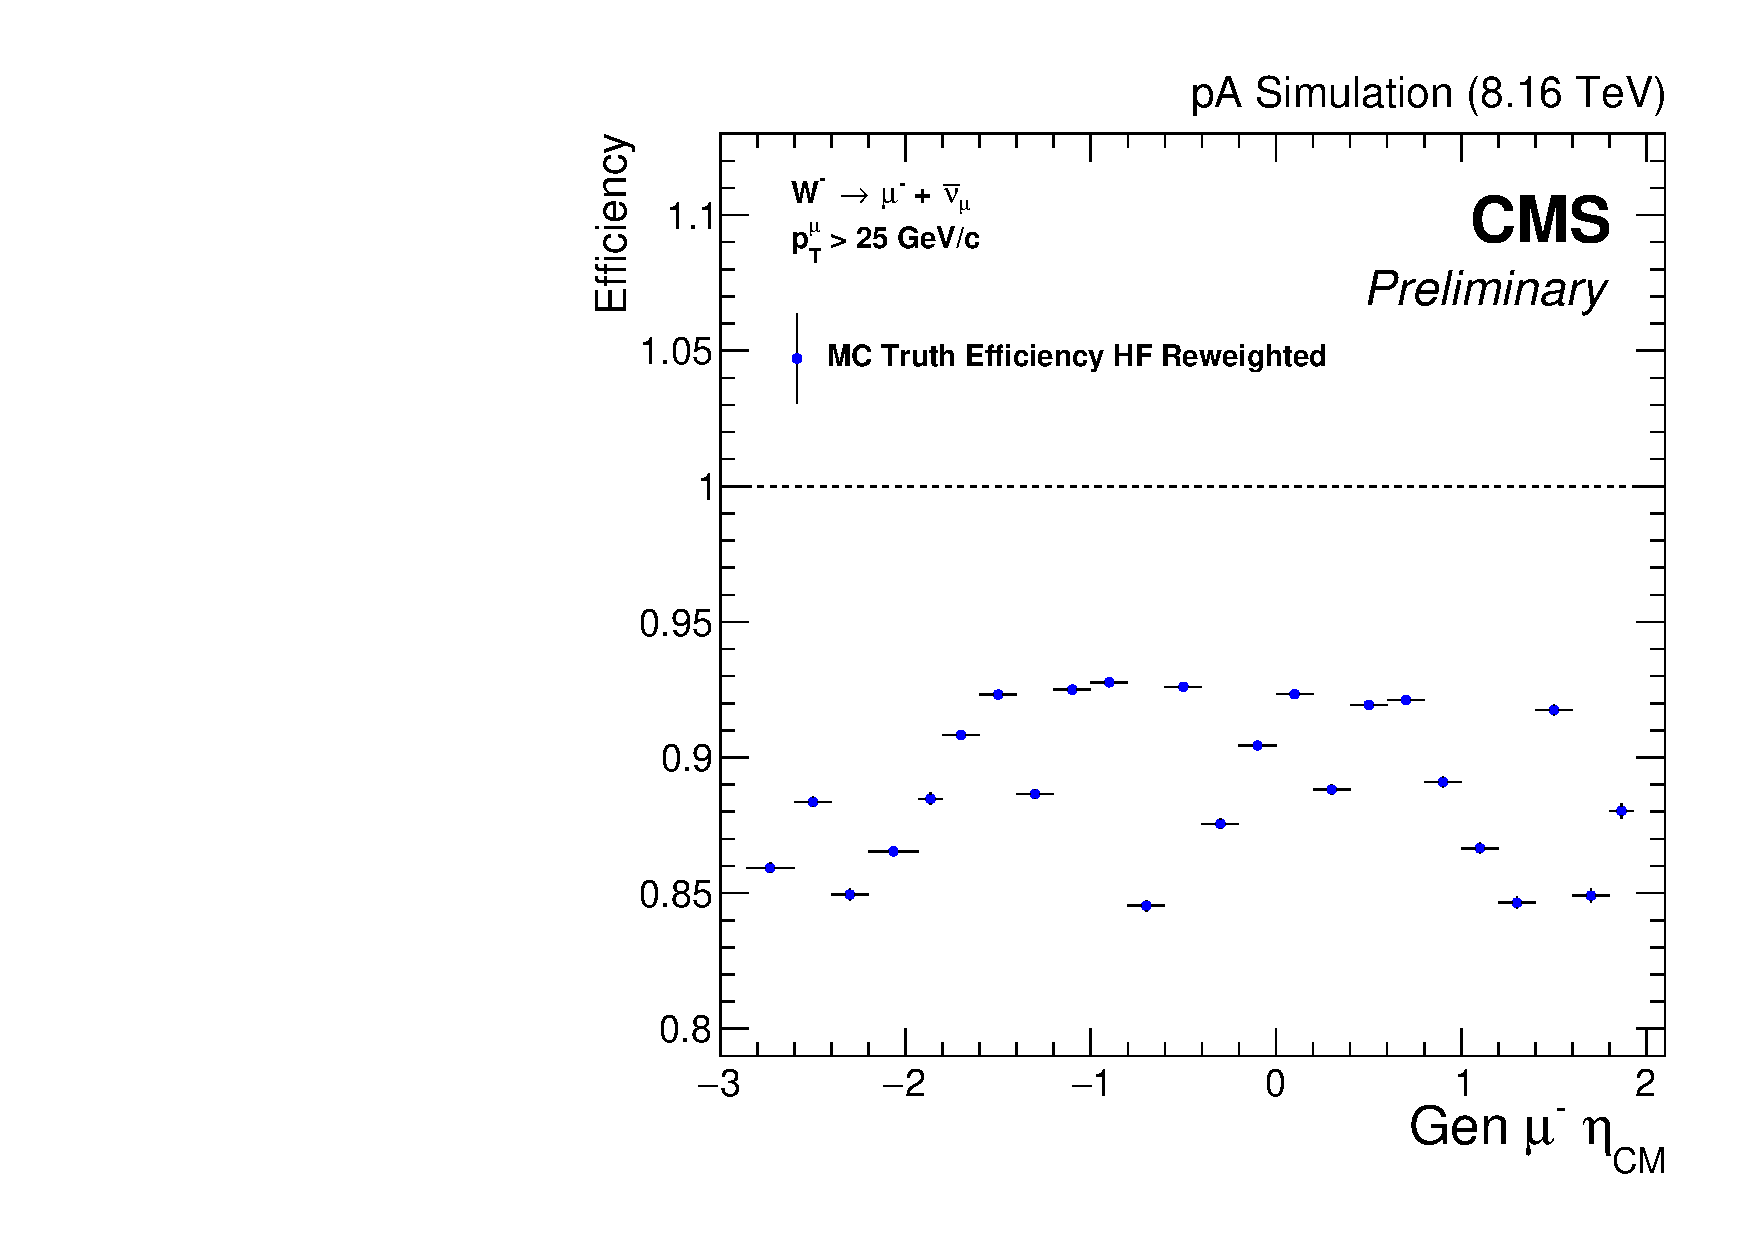
\includegraphics[width=0.45\textwidth]{Figures/WBoson/Analysis/Efficiency/Muon/PA/eff1D_EtaCM_MC_WToMuNu_PA_Minus_Total_HFCorrOnly}
   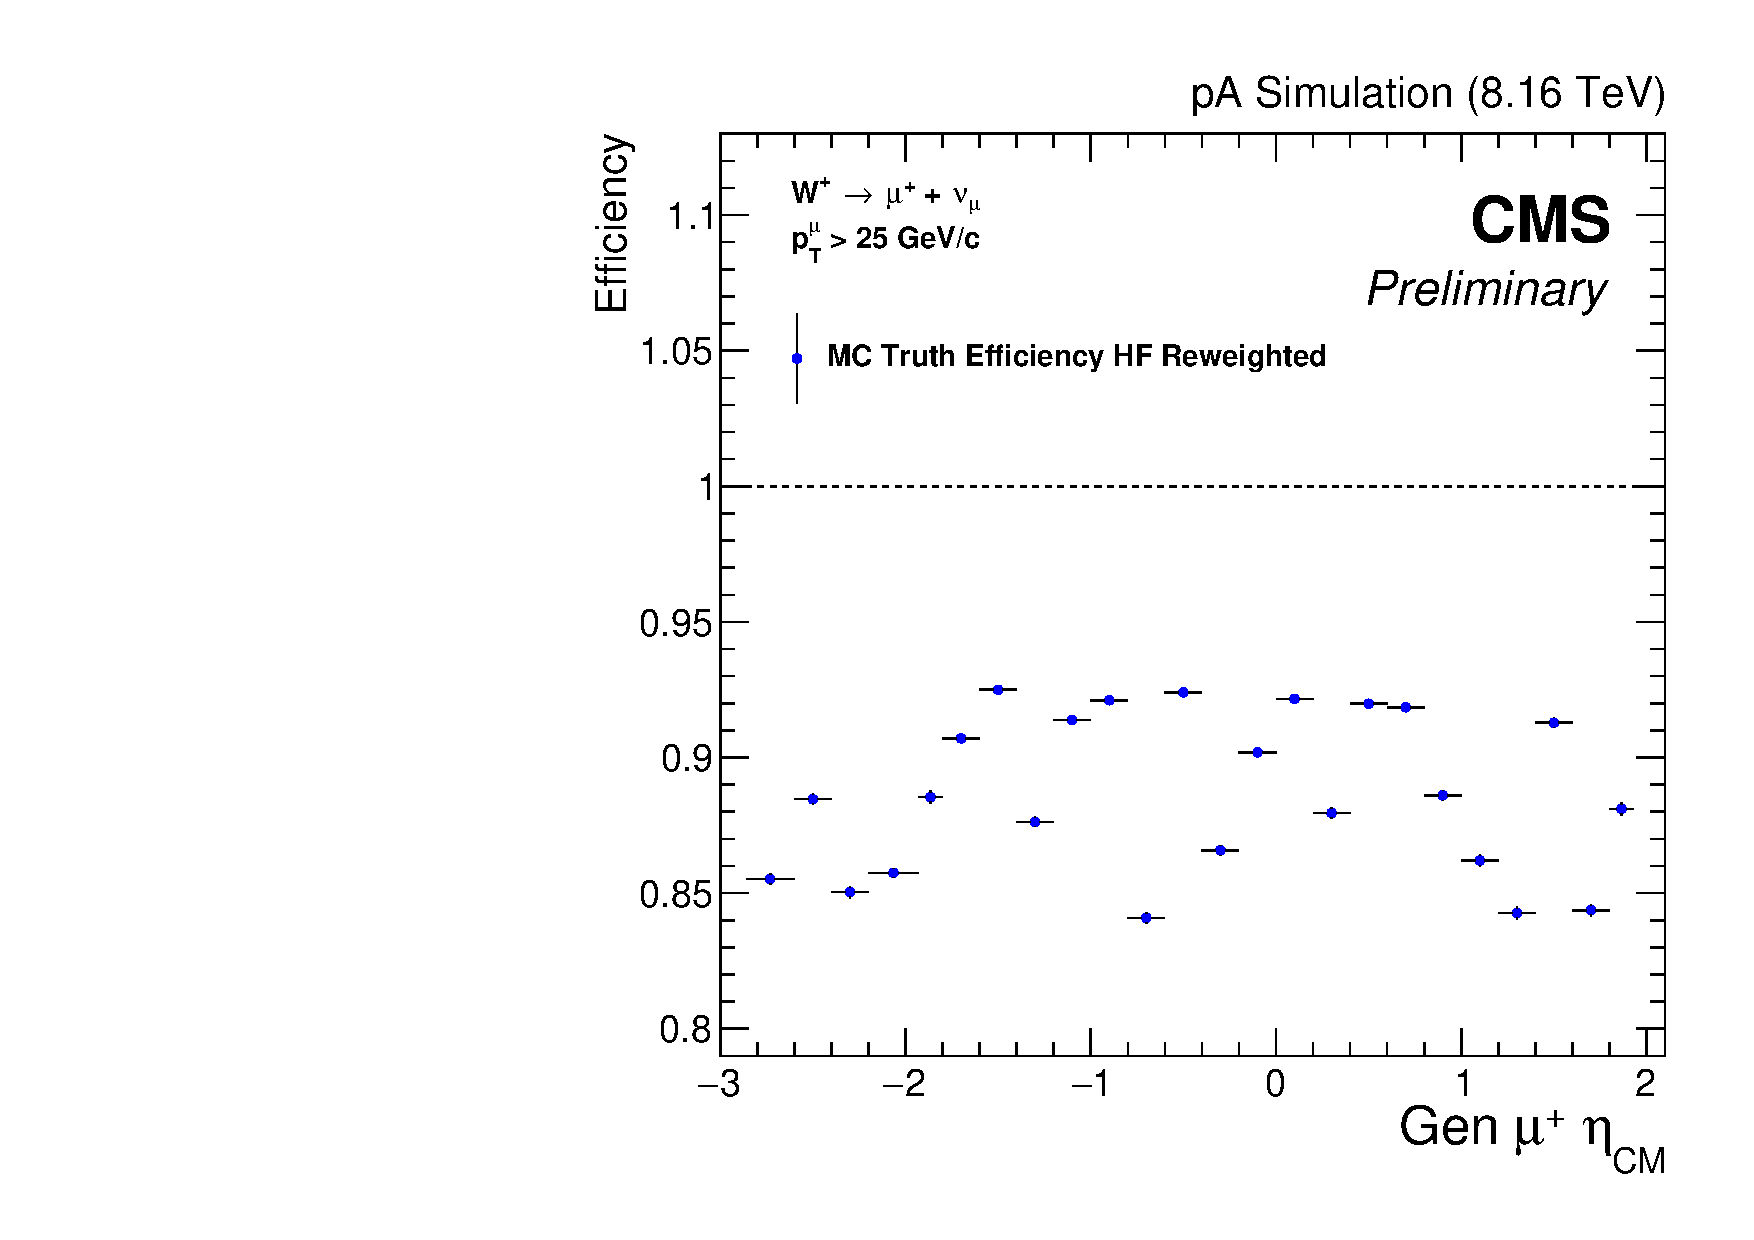
\includegraphics[width=0.45\textwidth]{Figures/WBoson/Analysis/Efficiency/Muon/PA/eff1D_EtaCM_MC_WToMuNu_PA_Plus_Total_HFCorrOnly}
 \end{center}
 \caption{Truth efficiency derived from \WToMuNu \POWHEG MC sample as a function of the generated muon $\eta_{CM}$, separated in negative (left) and positive (right) charged muons. The event activity of the MC samples have been reweighted. Plots corresponds to \eq{eq:MCTruthEfficiency}, and the \pPb and \Pbp MC efficiencies are combined according to \eq{eq:MCEfficiencyPA}. Only MC statistical errors are included.}
 \label{fig:MCTruthEfficiency}
\end{figure}

\begin{table}[h!]
  \centering
  \resizebox{\textwidth}{!}{
  \renewcommand{\arraystretch}{1.5}
  \begin{tabular}{|c|*4c|}
    \hline
    $\eta_{CM}$ Range & $\mu^{-}$ Truth Eff. & $\mu^{-}$ Reweighted Eff. & $\mu^{+}$ Truth Eff. & $\mu^{+}$ Reweighted Eff.\\
    \hline\hline
    -2.86 , -2.60 & $0.865 \pm 0.002$ & $0.859 \pm 0.002$ & $0.860 \pm 0.002$ & $0.855 \pm 0.002$\\
    \hline
    -2.60 , -2.40 & $0.890 \pm 0.002$ & $0.884 \pm 0.002$ & $0.889 \pm 0.002$ & $0.885 \pm 0.002$\\
    \hline
    -2.40 , -2.20 & $0.855 \pm 0.002$ & $0.849 \pm 0.002$ & $0.855 \pm 0.002$ & $0.850 \pm 0.002$\\
    \hline
    -2.20 , -1.93 & $0.871 \pm 0.001$ & $0.865 \pm 0.002$ & $0.864 \pm 0.002$ & $0.857 \pm 0.002$\\
    \hline
    -1.93 , -1.80 & $0.892 \pm 0.002$ & $0.885 \pm 0.002$ & $0.892 \pm 0.002$ & $0.885 \pm 0.002$\\
    \hline
    -1.80 , -1.60 & $0.913 \pm 0.001$ & $0.908 \pm 0.002$ & $0.914 \pm 0.001$ & $0.907 \pm 0.002$\\
    \hline
    -1.60 , -1.40 & $0.932 \pm 0.001$ & $0.923 \pm 0.002$ & $0.931 \pm 0.001$ & $0.925 \pm 0.001$\\
    \hline
    -1.40 , -1.20 & $0.892 \pm 0.002$ & $0.886 \pm 0.002$ & $0.883 \pm 0.002$ & $0.876 \pm 0.002$\\
    \hline
    -1.20 , -1.00 & $0.932 \pm 0.001$ & $0.925 \pm 0.001$ & $0.924 \pm 0.001$ & $0.914 \pm 0.002$\\
    \hline
    -1.00 , -0.80 & $0.935 \pm 0.001$ & $0.928 \pm 0.001$ & $0.930 \pm 0.001$ & $0.921 \pm 0.002$\\
    \hline
    -0.80 , -0.60 & $0.853 \pm 0.002$ & $0.845 \pm 0.002$ & $0.848 \pm 0.002$ & $0.841 \pm 0.002$\\
    \hline
    -0.60 , -0.40 & $0.934 \pm 0.001$ & $0.926 \pm 0.001$ & $0.931 \pm 0.001$ & $0.924 \pm 0.002$\\
    \hline
    -0.40 , -0.20 & $0.881 \pm 0.002$ & $0.876 \pm 0.002$ & $0.873 \pm 0.002$ & $0.866 \pm 0.002$\\
    \hline
    -0.20 , +0.00 & $0.912 \pm 0.001$ & $0.904 \pm 0.002$ & $0.909 \pm 0.001$ & $0.902 \pm 0.002$\\
    \hline
    +0.00 , +0.20 & $0.930 \pm 0.001$ & $0.923 \pm 0.002$ & $0.928 \pm 0.001$ & $0.922 \pm 0.002$\\
    \hline
    +0.20 , +0.40 & $0.896 \pm 0.002$ & $0.888 \pm 0.002$ & $0.887 \pm 0.002$ & $0.880 \pm 0.002$\\
    \hline
    +0.40 , +0.60 & $0.926 \pm 0.001$ & $0.919 \pm 0.002$ & $0.926 \pm 0.001$ & $0.920 \pm 0.002$\\
    \hline
    +0.60 , +0.80 & $0.926 \pm 0.001$ & $0.921 \pm 0.002$ & $0.926 \pm 0.001$ & $0.919 \pm 0.002$\\
    \hline
    +0.80 , +1.00 & $0.896 \pm 0.002$ & $0.891 \pm 0.002$ & $0.891 \pm 0.002$ & $0.886 \pm 0.002$\\
    \hline
    +1.00 , +1.20 & $0.873 \pm 0.002$ & $0.867 \pm 0.002$ & $0.868 \pm 0.002$ & $0.862 \pm 0.002$\\
    \hline
    +1.20 , +1.40 & $0.850 \pm 0.002$ & $0.846 \pm 0.002$ & $0.847 \pm 0.002$ & $0.843 \pm 0.002$\\
    \hline
    +1.40 , +1.60 & $0.920 \pm 0.002$ & $0.917 \pm 0.002$ & $0.917 \pm 0.001$ & $0.913 \pm 0.002$\\
    \hline
    +1.60 , +1.80 & $0.853 \pm 0.002$ & $0.849 \pm 0.003$ & $0.849 \pm 0.002$ & $0.844 \pm 0.002$\\
    \hline
    +1.80 , +1.93 & $0.882 \pm 0.002$ & $0.880 \pm 0.003$ & $0.883 \pm 0.002$ & $0.881 \pm 0.002$\\
    \hline
  \end{tabular}
  }
  \caption{Muon truth efficiency as a function of the generated muon $\eta_{CM}$, derived from the $\WToMuNu$ PA \POWHEG samples separated in negative and positive charged muons. The \pPb and \Pbp MC samples are combined as described in \sect{sec:CombiningBeamDirection}. Generated muons are required to be matched to reconstructed muons passing all analysis cuts. The event activity of the MC samples has been re-weighted. Results corresponds to \eq{eq:MCTruthEfficiency}}
  \label{tab:mcEfficiency_WToMu_PA}
\end{table}




\clearpage
\subsubsection{Corrected Efficiency}\label{sec:WBoson_Analysis_CorrectedEfficiency}

Even though the MC simulations produced by the CMS colaboration are very precise, they are still far from fully describing all the detector conditions observed in real data. In order to compensate for imperfections in the simulation-based efficiencies, a set of muon scale factors using the Tag-and-Probe method have been produced centrally by the HIN Dilepton group and approved by the Muon POG.

The \textit{Tag-and-Probe} (TnP) method \cite{Muon_TnP} is a data-driven technique widely used to compute efficiencies of physical objects, such as muons, produced from known mass resonances (e.g. \JPsi, \Z). One advantage of the TnP method is that it can be applied to both MC and real data, allowing to asses the differences between the data and MC efficiencies. For high \pt muons ($\pt > 15$~\GeVc), the \ZToMuMu decays are used to build a clean sample. In each event, one muon is classified as the "tag" if it has a $\pt > 15$~\GeVc and passes all the analysis cuts (trigger matching, isolation and identification), ensuring that it is a real muon, while the remaining muon is labelled as the "probe". Subsequently, the invariant mass distribution of the tag-probe dimuons is fitted in three cases: all pairs, failed pairs and passing pairs, depending on wether the probe muon passes or fails the selection criteria. The efficiency is calculated as a function of the probe \pt and $\eta_{LAB}$ in the laboratory frame by dividing the extracted yields of the passing pairs over all the pairs for various kinematic ranges of the probe. Finally, the TnP efficiencies in data and MC are compared, and the ratio of the two efficiencies is used to correct the simulations. More information about the \pPb TnP scale factors can be found in \cite{Muon_TnP_pPb}.

In this analysis, the MC truth efficiencies derived in \sect{sec:WBoson_Analysis_MCTruthEfficiency} are corrected by applying event by event the TnP scale factors as a function of $\eta_{LAB}$ and \pt. The TnP scale factors are extracted from the macro \href{https://github.com/CMS-HIN-dilepton/MuonAnalysis-TagAndProbe/blob/80X_HI/macros/tnp_weight.h}{\texttt{tnp\_weight.h}} as recommended by the HIN Dilepton group. The corrected muon efficiency is compared to the truth and the HF reweighted efficiencies in \fig{fig:CorrEfficiency_HFCorr}.

\begin{figure}[htb!]
 \begin{center}
   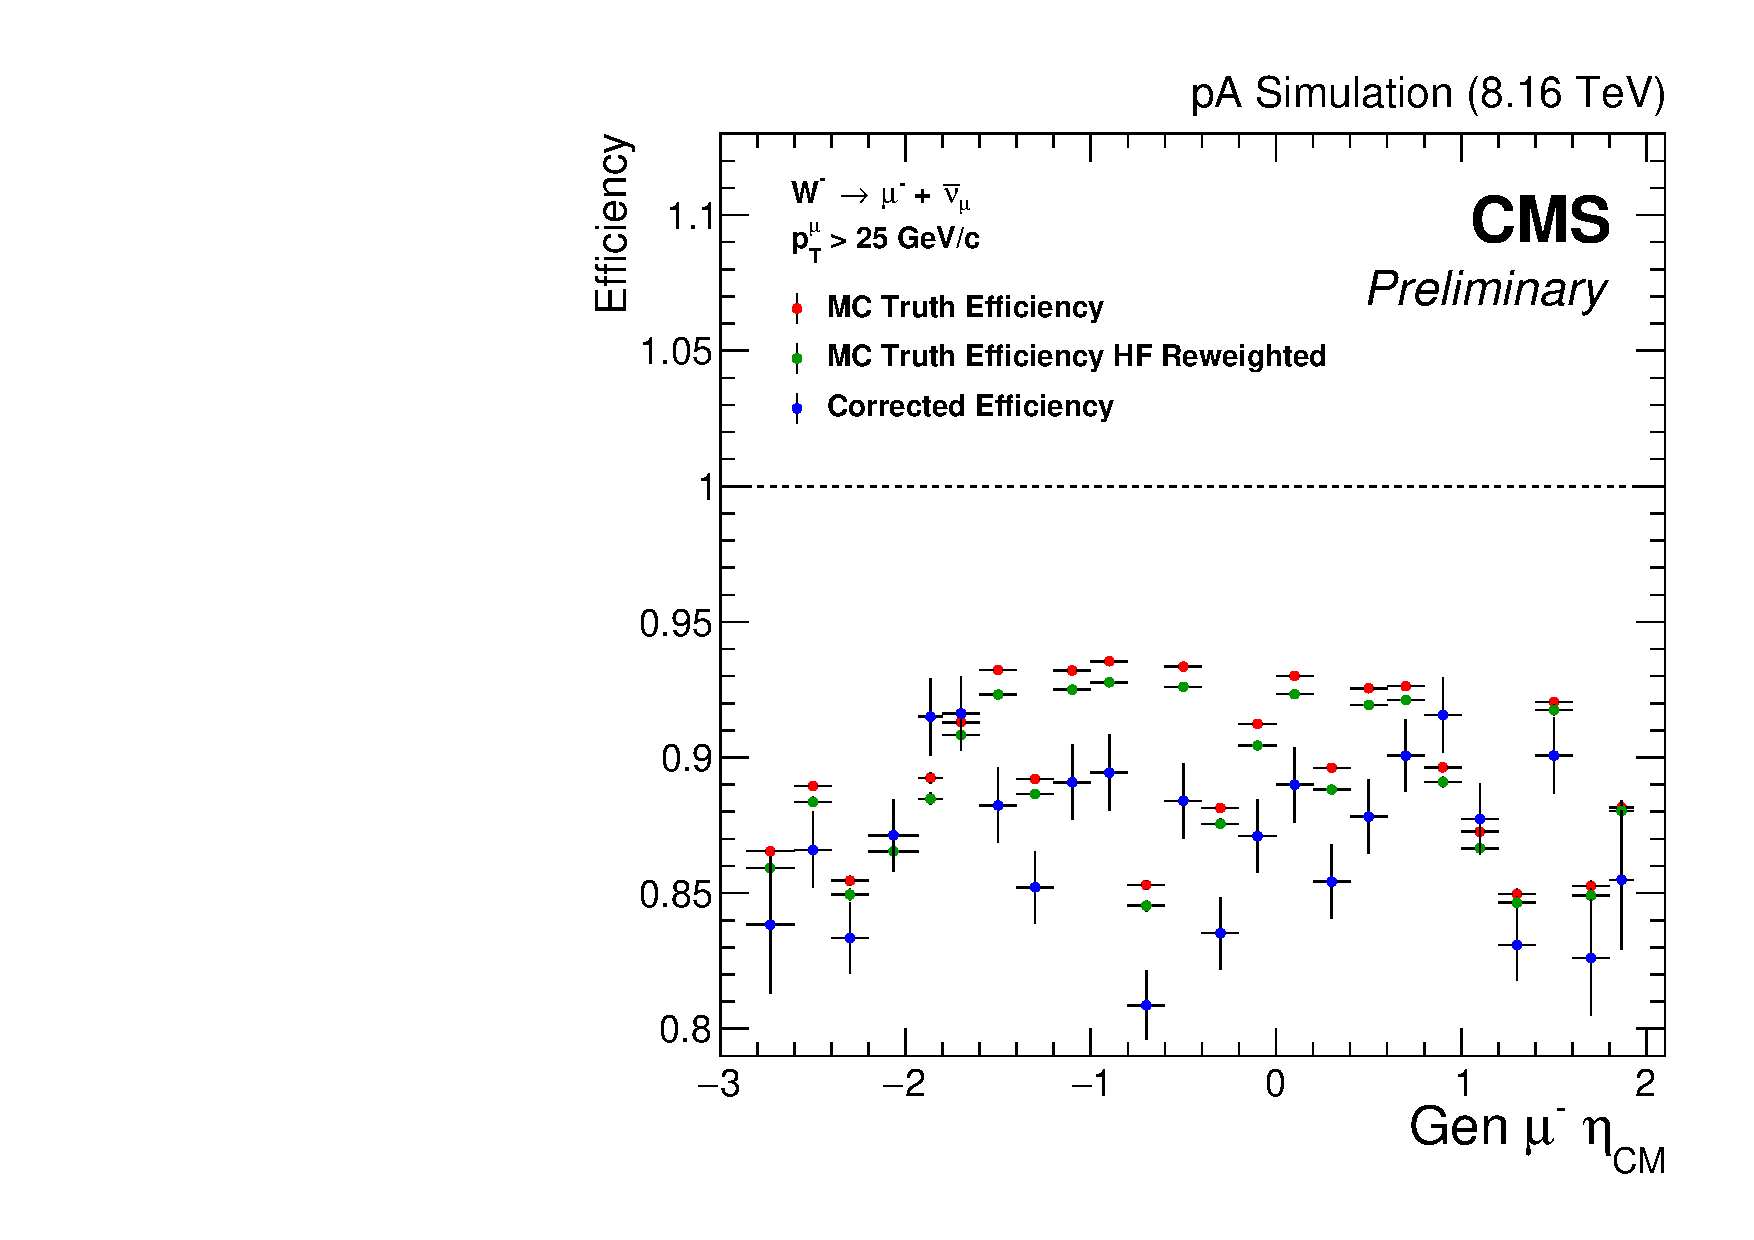
\includegraphics[width=0.45\textwidth]{Figures/WBoson/Analysis/Efficiency/Muon/PA/eff1D_EtaCM_MC_WToMuNu_PA_Minus_Total_HFCorr}
   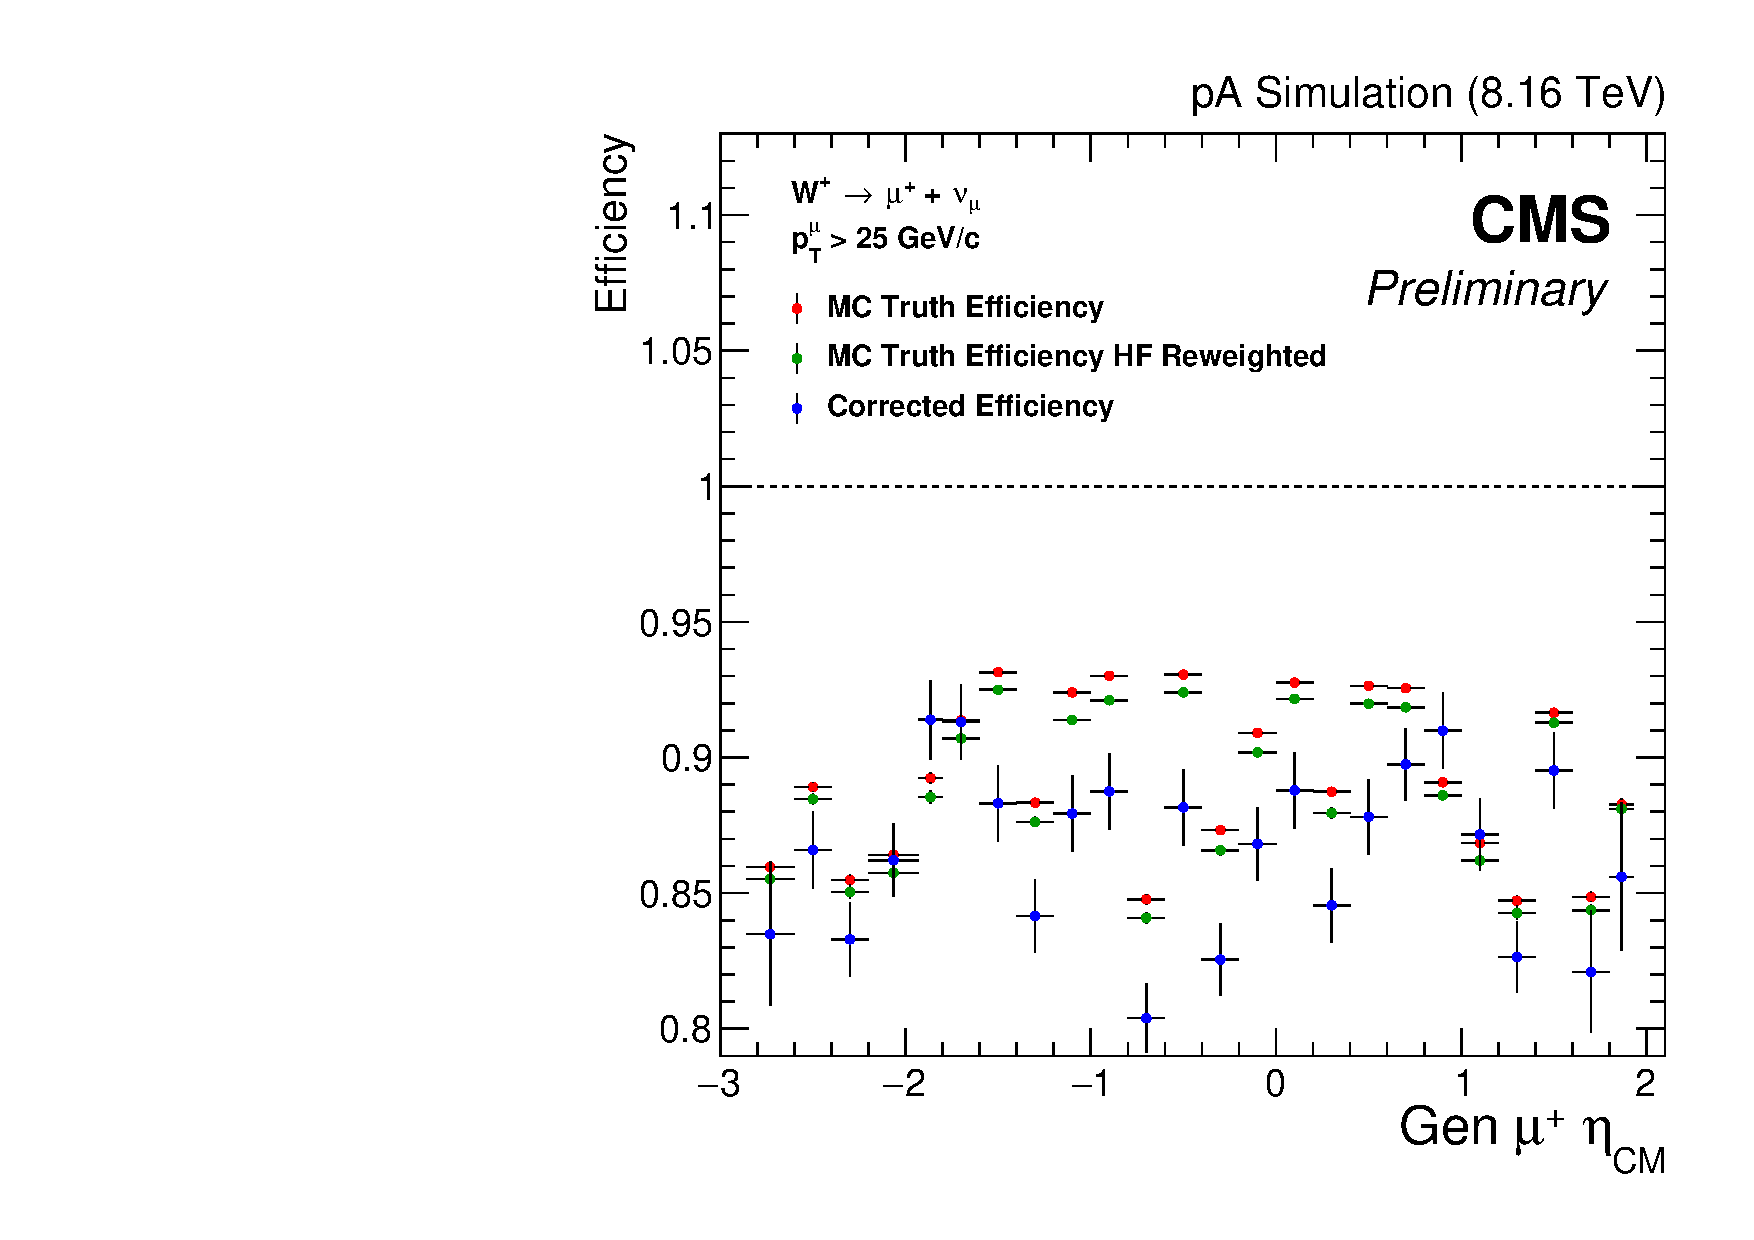
\includegraphics[width=0.45\textwidth]{Figures/WBoson/Analysis/Efficiency/Muon/PA/eff1D_EtaCM_MC_WToMuNu_PA_Plus_Total_HFCorr}
 \end{center}
 \caption{Muon efficiencies derived from \WToMuNu \POWHEG MC sample as a function of the generated muon $\eta_{CM}$, separated in negative (left) and positive (right) charged muons. The red, green and blue points represents the truth efficiency, the event activity reweighted efficiency and the corrected efficiency, respectively. The \pPb and \Pbp MC efficiencies are combined according to \eq{eq:MCEfficiencyPA}. The error bars of the corrected efficiency includes the total TnP uncertainties on top of the MC statitical uncertainty.}
 \label{fig:CorrEfficiency_HFCorr}
\end{figure}

The statistical and systematic components of the TnP correction uncertainties are derived by applying the different variations of the scale factors provided in the macro \href{https://github.com/CMS-HIN-dilepton/MuonAnalysis-TagAndProbe/blob/80X_HI/macros/tnp_weight.h}{\texttt{tnp\_weight.h}}. The set of variations can be summarized as follows:

\begin{enumerate}
   \item TnP statistical uncertainty:
   \begin{enumerate}
      \item For muon ID and isolation: 100 scale factor variations derived from toy MC.
      \item For trigger: Up and down $1 \sigma_{stat}$ variations.
   \end{enumerate}
   \item TnP systematic uncertainty:
   \begin{enumerate}
      \item For muon ID, isolation and trigger: Up and down by $1 \sigma_{syst}$ variations.
      \item For muon ID and isolation: Using the scale factor from the Data/MC bins instead of the one derived from fitting the ratio.
      \item For isolation: An uncertainty of {\bf 0.34\%} to account for the impact on the isolation efficiency of the different level of activity and pile-up between data and MC.
      \item For stand-alone muon reconstruction: An uncertainty of {\bf 0.6\%} to account for mismodelings in the STA efficiency.
   \end{enumerate}
\end{enumerate}


The uncertainties on the muon efficiency due to the TnP corrections are calculated in three different ways, as explained below.

\begin{enumerate}
   \item Taking the RMS between the 100 efficiencies corrected using the toy MC scale factors. Used in 1.a.
   \item Taking the maximum difference between the efficiency corrected using the nominal and the varied TnP scale factors. Used in 1.b, 2.a and 2.b.
   \item Applying the TnP scale factor uncertainty as a relative uncertainty on the corrected efficiency. Used in 2.c and 2.d.
\end{enumerate}

The statistical and systematic TnP uncertainties are summarized in \eq{eq:uncert_stat} and \eq{eq:uncert_syst}, respectively. The total TnP uncertainty is obtained by combining all of the uncertainties mentioned above, according to \eq{eq:uncert_tot}.

\begin{eqnarray}
    \Delta\epsilon^\text{stat} & = & \left( \left[\text{max} (|\epsilon^\text{stat, trg}_{+} - \epsilon_0|, |\epsilon^\text{stat, trg}_{-} - \epsilon_0|)\right]^2\right. \nonumber\\
     &&+ \left[ \text{std.dev.} \left( \epsilon^\text{stat, muID}_i \right) \right]^2 \nonumber\\
     &&+ \left.\left[ \text{std.dev.} \left( \epsilon^\text{stat, iso}_i \right) \right]^2 \right)^{-1/2} \label{eq:uncert_stat}
\end{eqnarray}
   
\begin{eqnarray}
    \Delta\epsilon^\text{syst}  & = &  \left(\left[\text{max} (|\epsilon^\text{syst, trg}_{+} - \epsilon_0|, |\epsilon^\text{syst, trg}_{-} - \epsilon_0|)\right]^2\right.\nonumber\\
    &&+ \left[\text{max} (|\epsilon^\text{syst, muID}_{+} - \epsilon_0|, |\epsilon^\text{syst, muID}_{-} - \epsilon_0|)\right]^2\nonumber\\
    &&+ \left[\text{max} (|\epsilon^\text{syst, iso}_{+} - \epsilon_0|, |\epsilon^\text{syst, iso}_{-} - \epsilon_0|)\right]^2\nonumber\\
    &&+ \left[\epsilon^\text{syst, MuID binned} - \epsilon_0\right]^2 + \left[\epsilon^\text{syst, iso binned} - \epsilon_0\right]^2\nonumber\\
    &&+ \left.\left[\Delta\epsilon^\text{syst, HF+PU}\right]^2 + \left[\Delta\epsilon^\text{syst, STA}\right]^2\right)^{-1/2} \label{eq:uncert_syst}
\end{eqnarray}

\begin{equation}
    \Delta\epsilon^\text{tot}  =  \sqrt{ (\Delta\epsilon^\text{stat})^2 + (\Delta\epsilon^\text{syst})^2 } \label{eq:uncert_tot}
\end{equation}

The TnP corrected efficiencies including their total uncertainties are shown in \tab{tab:corrEfficiency_WToMu_PA} and \fig{fig:CorrEfficiency}. The uncertainties on the corrected efficiencies due to each TnP scale factor component are presented from \tab{tab:tnpSystUncertainty_WToMu_Plus_PA} to \tab{tab:tnpStatUncertainty_WToMu_Minus_PA}.

\begin{figure}[htb!]
 \begin{center}
   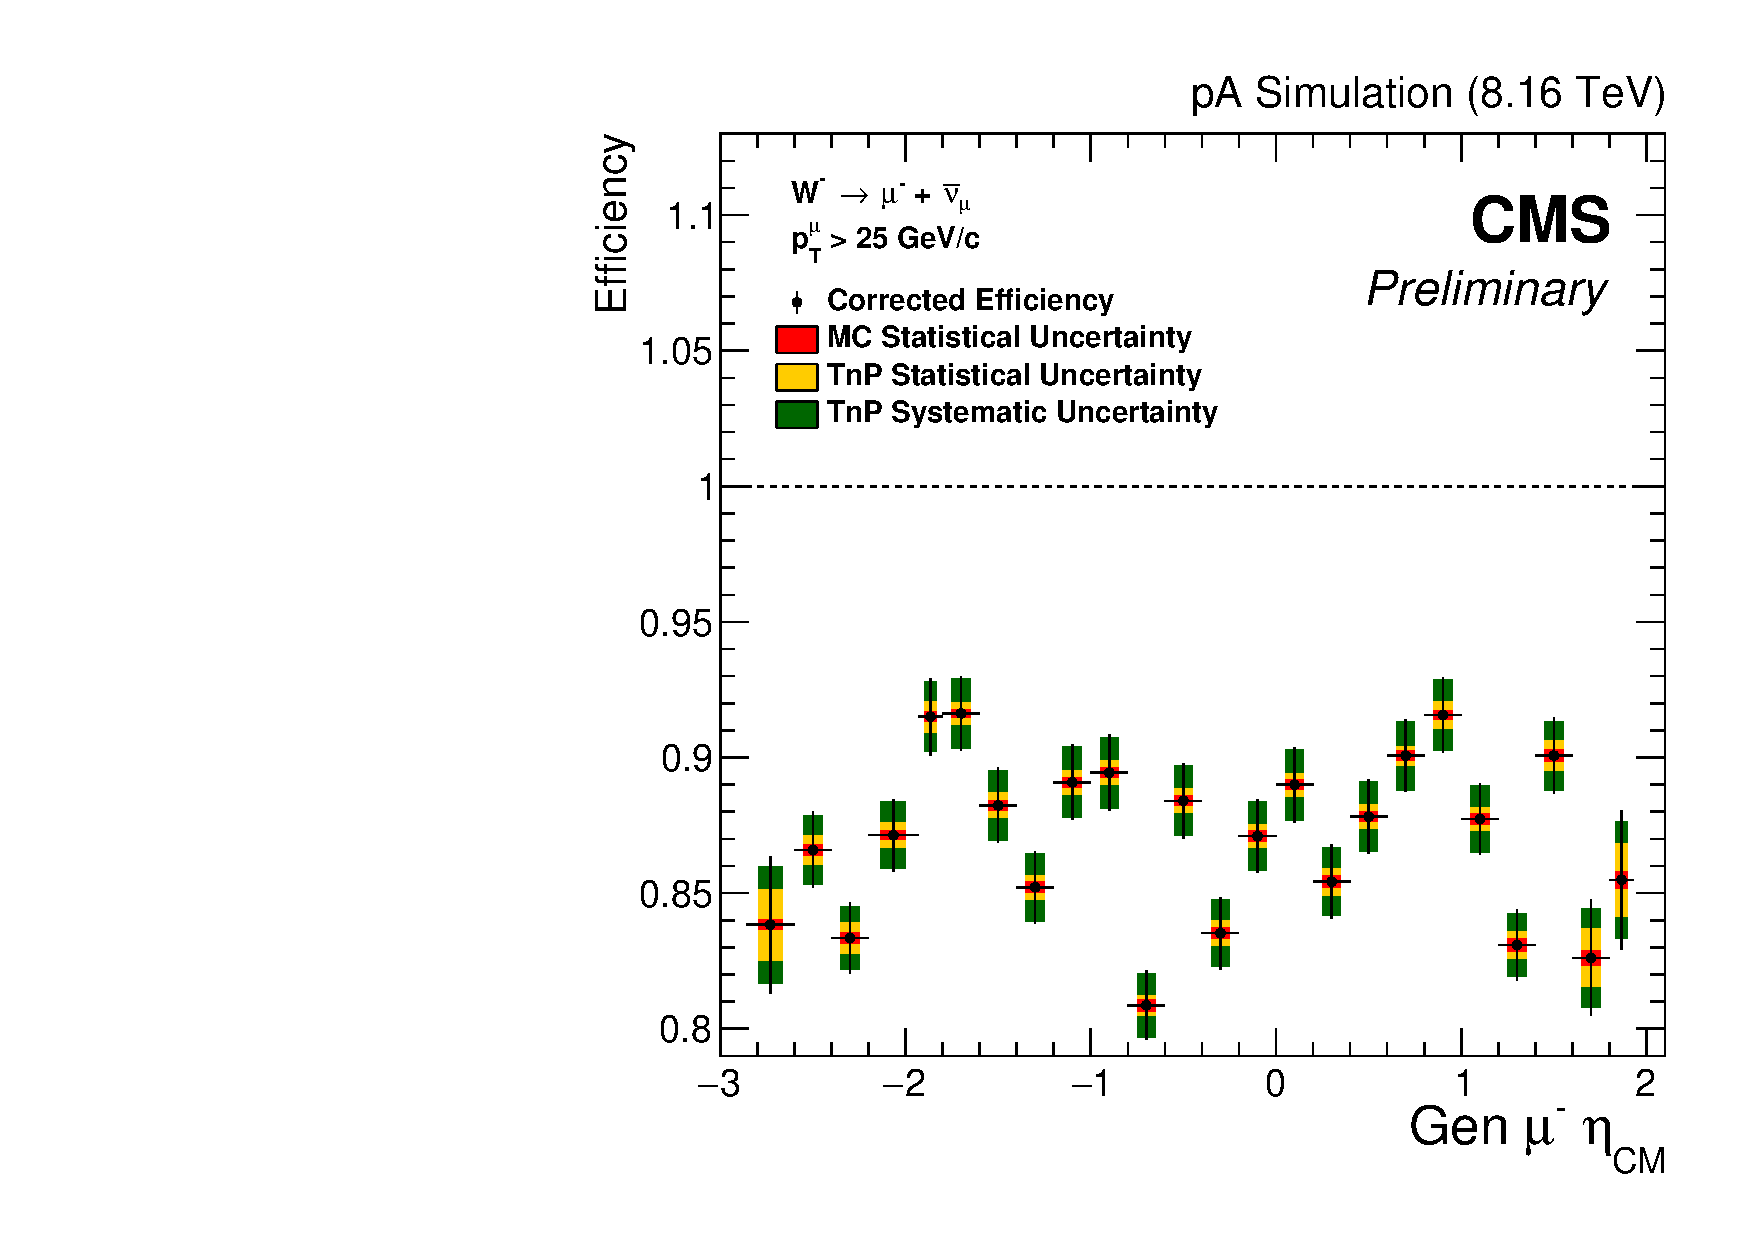
\includegraphics[width=0.45\textwidth]{Figures/WBoson/Analysis/Efficiency/Muon/PA/eff1D_EtaCM_MC_WToMuNu_PA_Minus_Total_TnP_Nominal}
   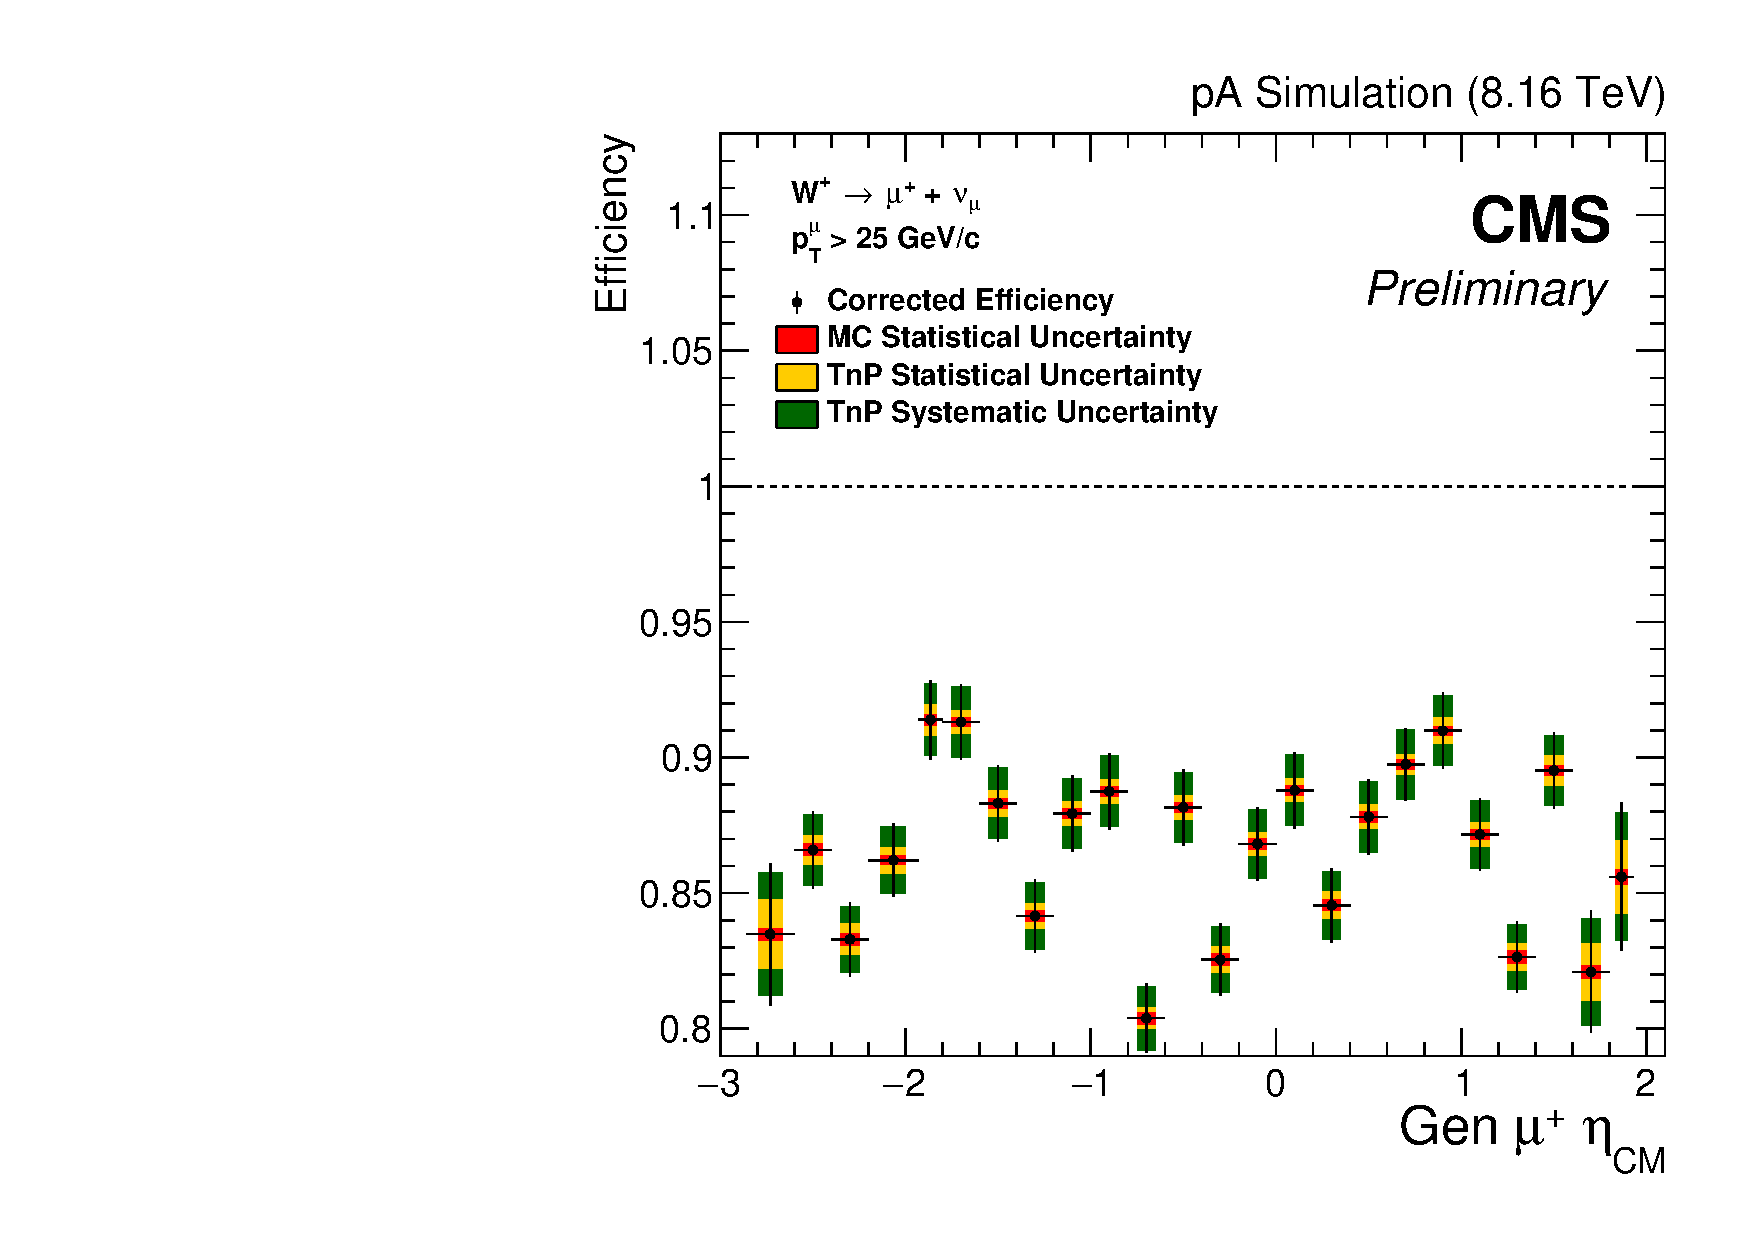
\includegraphics[width=0.45\textwidth]{Figures/WBoson/Analysis/Efficiency/Muon/PA/eff1D_EtaCM_MC_WToMuNu_PA_Plus_Total_TnP_Nominal}
 \end{center}
 \caption{Muon corrected efficiency derived from \WToMuNu \POWHEG MC sample as a function of the generated muon $\eta_{CM}$, separated in negative (left) and positive (right) charged muons. The muon efficiency has been corrected by applying the Tag and Probe scale factors event by event. The red, yellow and green boxes represents the uncertainty on the efficiency due to the MC statistics, TnP statistics and TnP systematics, respectively. The \pPb and \Pbp MC efficiencies are combined according to \eq{eq:MCEfficiencyPA}.}
 \label{fig:CorrEfficiency}
\end{figure}

\begin{table}[h!]
  \centering
  \renewcommand{\arraystretch}{1.5}
  \begin{tabular}{|c|*2c|}
    \hline
    $\eta_{CM}$ Range & $\mu^{-}$ Corrected Eff. & $\mu^{+}$ Corrected Eff.\\
    \hline\hline
    -2.86 , -2.60 & $0.838 \pm 0.002 \pm 0.025 \textrm{ (tnp)}$ & $0.835 \pm 0.002 \pm 0.026 \textrm{ (tnp)}$\\
    \hline
    -2.60 , -2.40 & $0.866 \pm 0.002 \pm 0.014 \textrm{ (tnp)}$ & $0.866 \pm 0.002 \pm 0.014 \textrm{ (tnp)}$\\
    \hline
    -2.40 , -2.20 & $0.833 \pm 0.002 \pm 0.013 \textrm{ (tnp)}$ & $0.833 \pm 0.002 \pm 0.013 \textrm{ (tnp)}$\\
    \hline
    -2.20 , -1.93 & $0.871 \pm 0.002 \pm 0.013 \textrm{ (tnp)}$ & $0.862 \pm 0.002 \pm 0.013 \textrm{ (tnp)}$\\
    \hline
    -1.93 , -1.80 & $0.915 \pm 0.002 \pm 0.014 \textrm{ (tnp)}$ & $0.914 \pm 0.002 \pm 0.014 \textrm{ (tnp)}$\\
    \hline
    -1.80 , -1.60 & $0.916 \pm 0.002 \pm 0.013 \textrm{ (tnp)}$ & $0.913 \pm 0.002 \pm 0.014 \textrm{ (tnp)}$\\
    \hline
    -1.60 , -1.40 & $0.882 \pm 0.002 \pm 0.014 \textrm{ (tnp)}$ & $0.883 \pm 0.002 \pm 0.014 \textrm{ (tnp)}$\\
    \hline
    -1.40 , -1.20 & $0.852 \pm 0.002 \pm 0.013 \textrm{ (tnp)}$ & $0.842 \pm 0.002 \pm 0.013 \textrm{ (tnp)}$\\
    \hline
    -1.20 , -1.00 & $0.891 \pm 0.002 \pm 0.014 \textrm{ (tnp)}$ & $0.879 \pm 0.002 \pm 0.014 \textrm{ (tnp)}$\\
    \hline
    -1.00 , -0.80 & $0.894 \pm 0.002 \pm 0.014 \textrm{ (tnp)}$ & $0.887 \pm 0.002 \pm 0.014 \textrm{ (tnp)}$\\
    \hline
    -0.80 , -0.60 & $0.809 \pm 0.002 \pm 0.012 \textrm{ (tnp)}$ & $0.804 \pm 0.002 \pm 0.012 \textrm{ (tnp)}$\\
    \hline
    -0.60 , -0.40 & $0.884 \pm 0.002 \pm 0.014 \textrm{ (tnp)}$ & $0.882 \pm 0.002 \pm 0.014 \textrm{ (tnp)}$\\
    \hline
    -0.40 , -0.20 & $0.835 \pm 0.002 \pm 0.013 \textrm{ (tnp)}$ & $0.826 \pm 0.002 \pm 0.013 \textrm{ (tnp)}$\\
    \hline
    -0.20 , +0.00 & $0.871 \pm 0.002 \pm 0.013 \textrm{ (tnp)}$ & $0.868 \pm 0.002 \pm 0.013 \textrm{ (tnp)}$\\
    \hline
    +0.00 , +0.20 & $0.890 \pm 0.002 \pm 0.014 \textrm{ (tnp)}$ & $0.888 \pm 0.002 \pm 0.014 \textrm{ (tnp)}$\\
    \hline
    +0.20 , +0.40 & $0.854 \pm 0.002 \pm 0.013 \textrm{ (tnp)}$ & $0.845 \pm 0.002 \pm 0.013 \textrm{ (tnp)}$\\
    \hline
    +0.40 , +0.60 & $0.878 \pm 0.002 \pm 0.014 \textrm{ (tnp)}$ & $0.878 \pm 0.002 \pm 0.014 \textrm{ (tnp)}$\\
    \hline
    +0.60 , +0.80 & $0.901 \pm 0.002 \pm 0.013 \textrm{ (tnp)}$ & $0.897 \pm 0.002 \pm 0.013 \textrm{ (tnp)}$\\
    \hline
    +0.80 , +1.00 & $0.916 \pm 0.002 \pm 0.014 \textrm{ (tnp)}$ & $0.910 \pm 0.002 \pm 0.014 \textrm{ (tnp)}$\\
    \hline
    +1.00 , +1.20 & $0.877 \pm 0.002 \pm 0.013 \textrm{ (tnp)}$ & $0.872 \pm 0.002 \pm 0.013 \textrm{ (tnp)}$\\
    \hline
    +1.20 , +1.40 & $0.831 \pm 0.002 \pm 0.013 \textrm{ (tnp)}$ & $0.826 \pm 0.002 \pm 0.013 \textrm{ (tnp)}$\\
    \hline
    +1.40 , +1.60 & $0.901 \pm 0.002 \pm 0.014 \textrm{ (tnp)}$ & $0.895 \pm 0.002 \pm 0.014 \textrm{ (tnp)}$\\
    \hline
    +1.60 , +1.80 & $0.826 \pm 0.003 \pm 0.021 \textrm{ (tnp)}$ & $0.821 \pm 0.002 \pm 0.022 \textrm{ (tnp)}$\\
    \hline
    +1.80 , +1.93 & $0.855 \pm 0.003 \pm 0.025 \textrm{ (tnp)}$ & $0.856 \pm 0.003 \pm 0.027 \textrm{ (tnp)}$\\
    \hline
  \end{tabular}
  \caption{Muon corrected efficiency as a function of the generated muon $\eta_{CM}$, derived from the $\WToMuNu$ PA \POWHEG samples separated in negative and positive charged muons.  The \pPb and \Pbp MC samples are combined as described in \sect{sec:CombiningBeamDirection}. Generated muons are required to be matched to reconstructed muons passing all analysis cuts. The muon efficiency has been corrected by applying the Tag and Probe scale factors event by event. The label "tnp" represent the TnP total uncertainty.}
  \label{tab:corrEfficiency_WToMu_PA}
\end{table}





% END OF SUBSECTION
\clearpage
